%
% File acl2019.tex
%
%% Based on the style files for ACL 2018, NAACL 2018/19, which were
%% improvements
%%  taken from the NAACL-2016 style
%% Based on the style files for ACL-2014, which were, in turn,
%% based on ACL-2013, ACL-2012, ACL-2011, ACL-2010, ACL-IJCNLP-2009,
%% EACL-2009, IJCNLP-2008...
%% Based on the style files for EACL 2006 by 
%%e.agirre@ehu.es or Sergi.Balari@uab.es
%% and that of ACL 08 by Joakim Nivre and Noah Smith

\documentclass[11pt,a4paper]{article}
\usepackage[hyperref]{acl2019}
\usepackage{times}
\usepackage{latexsym}
\usepackage{mdframed}
\usepackage{verbatim}
\usepackage{xcolor}
\usepackage{graphicx}
\usepackage{amsmath}
\usepackage{url}
\usepackage{multirow}

\aclfinalcopy % Uncomment this line for the final submission
%\def\aclpaperid{***} %  Enter the acl Paper ID here

%\setlength\titlebox{5cm}
% You can expand the titlebox if you need extra space
% to show all the authors. Please do not make the titlebox
% smaller than 5cm (the original size); we will check this
% in the camera-ready version and ask you to change it back.

\newcommand\BibTeX{B\textsc{ib}\TeX}

\title{Improving SoTA: Token-level Extractive Neural Document Summarization}

\author{Haojun Li \\
  \texttt{haojun@stanford.edu}\\
  \texttt{Department of Computer Science, Stanford University}
}
\date{}

\begin{document}
\maketitle
\begin{abstract}
	Neural Document Summarization has seen dramatic improvements over traditional methods, and recent advancements in contextual pretrained embeddings allow models to do much better in this task. Abstractive methods achieve higher coherency, but with less accurate content selection. Extractive methods are limited to sentence selection with few experiments on token selection. This work proposes a new method in labeling source tokens' membership in target summary, and show that training a simple linear classifier on top of Bert achieves better ROUGE scores than attained by previous papers, including current state-of-the-art sentence-selection method that uses Bert. By varying threshold, this model can be used as either a keyword extraction model or full summarization model. Though the generated summaries are not as coherent as abstractive methods, the labeling method and the model provides a content selector which would improve future abstractive methods in accurately selecting content.
\end{abstract}

\section{Introduction}
	The Document summarization task is defined as compressing or summarizing a long article of several hundred tokens into a short paragraph of less than 100 tokens. This task is viewed as one of the several general NLU tasks that tests NLU systems on their ability to understand texts. In the age of twitter and short attention span of readers, document summarization is more relevant than ever. Many news sources have even begun including a three sentence summary on top of their news article that "summarizes" or "highlights" the article.  
	
	There are currently 2 main ways of achieving document summarization: extractive and abstractive summarization. Extractive summarization casts this problem as a sentence-level binary classification problem where the model aims to predict source sentence membership in a human written target summary \cite{SummaRuNNer} \cite{al2018hierarchical} \cite{bert-sum}. This method works fairly well since real human summaries tends to also include several sentences picked and paraphrased from the source document, but it is constrained by the fact that sentences has to be copied whole from the source. Abstractive summarization aims to solve this coherency problem by casting this problem as a translation task where the model reads in the source document and generates a summary with novel words.\cite{bottom-up} \cite{lead} \cite{dca} \cite{pointer-generator} This method usually generates more coherent summaries than extractive methods, and are sometimes able to paraphrase the source document with novel words. However, it also introduce more problems such as inaccurate factual representation and repeated paraphrasing. 
	
	Since about 83\% of the tokens in the target summary are part of the source summary, we cast the document summarization task as a token-level extractive summarization task. Essentially, we tag each token in the source document that will be part of the target summary in a novel way, and use contextual embedding (Bert)\cite{bert} together with other models to predict source token membership in the target summary. We will show that the method described in this report not only improve upon both extractive sentence membership selection methods and abstractive seq-seq methods, but are also comparable to or better than current state of the art systems. We will work on the unanonymized CNN/DailyMail dataset following \citet{pointer-generator}. Section 2 summarizes several recent related papers in this area. Section 3 describe the dataset and metrics of evaluation. Section 4 describe the token selection method. Section 5 describe the models used to predict token membership. Section 6 describes experimental parameters. Section 7 describes results, strength and weakness of the model. Section 8 concludes the report and describes future works.

\section{Related Works}
Document summarization tasks has been around for a long time. The first introduction of a popular document summarization dataset is from DUC 2004. The dataset contains 500 documents with on average 35.6 tokens and summaries with 10.4 tokens.\footnote{Information obtained from \url{http://nlpprogress.com/english/summarization.html}} Since the dataset is quite small, it is mostly used for evaluating neural networks trained on other richer datasets. Later on, Gigaword emerged as another viable dataset for neural summarization systems since it has a lot more training examples (around 4 million articles). This dataset is first used by \citet{rush} to train an attention based neural network for abstractive summarization. In that paper, they described a method that allows them to use attention as an alignment mechanism to align source tokens to target summary tokens. This has greatly improved upon non-neural models, but still unable to achieve human-level performance. The reason seems to be that even though the network is great at predicting keywords, it sometimes reorder the words in the wrong way. Later methods use more and more complicated models as well as incorporate templates to guide seq-seq models \cite{rethink}. 

%While more and more researchers are using neural methods for abstractive and extractive summarization, non-neural methods that combines traditional NLU tasks such as dependency tree parsing, sentence clustering with custom distance metrics, coreference resolution to generate summaries. \cite{unsuper} is one such paper where they combined several traditional NLU methods to generate summaries. However, their system are only able to cluster sentences and summarize sentences within the cluster, and they did not describe a way to correctly pick sentences after summarization is done. Thus, their method does not seem to be able to generalize to longer documents.

Since recurrent neural networks are notoriously bad on tasks involving longer sequences, most models work well in compressing already short sentences or generating a headline from a paragraph of around 40 tokens. With recent exponential increases in computing power, researchers began tackling summarization tasks that involves longer sequences. The first neural summarization paper that uses seq-seq neural architecture with attention is \citet{lead}. They first noted that off-the-shelf seq-seq neural networks used for Machine Translation (MT) already out performs state-of-the-art systems at the time without any modifications. Then, they described several methods in enhancing the word2vec embeddings and used an encoder-decoder model with attention to generate a coherent summary. To deal with rare words, they had a "copy distribution" which attempts to predict which source token to copy when encountering an UNK token (unknown vocabulary) in decoding. They achieved state-of-the-art results while operating on the anonymized\footnote{All entities in the document is replaced with @entity tags} CNN/DailyMail dataset, which has 10x longer source sentences than other datasets. 

This advancement in neural document summarization sparked huge interest in long document summarization research. A later paper \cite{pointer-generator} designed a similar network to not only copy words when encountering an UNK token, but allows the network to copy in any words at anytime when decoding by calculating a "generation probability". This method (enhanced with a "coverage" loss to prevent repeated sentences) worked better than basic seq-seq models, but still has limitations such as factually incorrect paraphrases. The author noted that the model learned to mostly copy words from the source document, and still unable to beat the extractive summary methods in terms of ROUGE scores. They also operated on the unanonymized CNN/DailyMail dataset, saying it as a harder and more interesting problem. Other paper attempts to improve upon this pointer generator network with a content selector first \cite{bottom-up}. Essentially, they train a separate content selector that selects keywords from the source document, and biases the "copy distribution" to only copy selected keywords. The content selector was trained on labels selected by matching source tokens with target summary tokens, and the first occurrence of the target token in the source is tagged. This paper is the most relatable paper to this project, since we also define a content selector but uses a different tagging criteria.

Abstractive summarization methods described above are the most interesting and exciting, while extractive methods seems to work better.  \citet{SummaRuNNer} later authored another paper but instead of using an abstractive seq-seq model, they described a model that use recurrent networks to predict sentence membership in the source document. This beat the state-of-the-art results again by correctly selecting sentences from the source document to be included in the summary. Notably, this paper beat their own abstractive summary results and pointer-generator results, since most of the sentences from the target summary are, indeed, directly copied or paraphrased from the source document. Other paper explored hierarchical attention mechanisms \cite{al2018hierarchical} and achieved slightly better results. Recent advancements in contextual embeddings allowed researchers to get even better results than previously possible. \citet{bert-sum} is the most recent paper that combines Bert with other architectures to do the same sentence-selection style extractive summary. Several other advancements has also been made in Reinforcement Learning (RL) applied to document summarization. \citet{dca} is one such example that is cited across papers. The author cast the problem as a RL problem and incorporated reward mechanisms to allow agents to make better decisions than simply maximizing the log likelihood of the prediction.


\section{Dataset and Metric}
Following all previous papers, we will use the unanonymized version of CNN/DailyMail dataset introduced as part of \citet{pointer-generator}. This is a dataset that contains news articles with an average of 781 tokens in the source documents and on average 56 tokens in the target multi-sentence summaries. We used the same preprocessing code as that paper\footnote{Preprocessing code can be found at \url{https://github.com/abisee/cnn-dailymail}}. Then, instead of splitting the data as they did, we split the data 90/5/5 for training, development, and test following \citet{bert-sum}. Since we need to use Bert as our contextual embedding extractor, we lower-cased all words within both the source document and target summary and tokenized the source and target documents again according to Bert's specification\footnote{we used the HuggingFace Bert pytorch library to do our Bert tokenization and training. HuggingFace's code can be found at \url{https://github.com/huggingface/pytorch-pretrained-BERT}}. Note that Bert tokenizes data differently from how most other paper tokenizes data. Thus, results from this report shouldn't be directly quoted to compare with other papers since tokenization is different. However, when we evaluate our model, we attempt to reconstruct the summary as humanly readable as possible to make our evaluation comparable to other papers.

The metric used in this report will be the same metrics used in all other papers, namely the ROUGE-1, ROUGE-2, ROUGE-L scores. They corresponds to uni-gram overlap, bi-gram overlap, and longest common sequence overlap between predicted summaries and gold summaries. Following previous papers, we will report the final test F-1 score of these metrics, while doing some analysis on precision and recall. Note that this metric is not the best metric for evaluating document summarization systems since it does not take into account the coherence and grammaticality of the generated summaries. Thus, even if a generated summary has high uni-gram and bi-gram overlaps with gold summaries, they could have been reordered in a way that is neither factually correct nor coherent. Thus, abstractive summarization methods tends to do worse in terms of ROUGE scores than extractive summarization methods while generating more grammatically coherent summaries. Instead of using PyRouge as used by previous papers, we will use the \textbf{rouge} package\footnote{A description of the library can be found at \url{https://pypi.org/project/rouge/}} for faster evaluation.


\section{Token Selection Method}
Borrowing the sequence tagging idea from \citet{bottom-up}, we cast the summarization problem as a sequence tagging problem. In the original paper, their content selection method is:
\begin{quote}
	We define a word xi as copied if (1) it is part of the longest possible sub-sequence of tokens $s = x_{i-j:i:i+k}$, for integers $j \leq i$; $k \leq (n-i)$,if $s \in x$ and  $s \in y$, and (2) there exists no earlier sequence $u$ with $s = u$.
\end{quote}

 \begin{table}[t]
	\begin{tabular}{@{}|l|@{}}
		\hline
		\begin{minipage}{.9\linewidth}
			\vspace{.1in}
			\textbf{Source:} \\
			"[...] the royal canadian mounted police yesterday arrested chiheb esseghaier , 30 , of montreal , and raed jaser , 35 , of \textcolor{blue}{toronto} . [...] police were later seen raiding \textcolor{purple}{jaser ' s house in} northern \textcolor{green}{toronto} , carrying away material which could be used as evidence in the suspects ' prosecution . [...]
		\end{minipage}\\ \hline
		
		\begin{minipage}{.9\linewidth}
			\vspace{.1in}
			\textbf{Target:}\\
			"chiheb esseghaier , 30 , and raed jaser , 35 , were arrested yesterday . suspected received orders and got guidance from al qaeda leader in iran . planned to target new york - bound trains in toronto . \textcolor{orange}{jaser ' s house in toronto} raided by police and evidence removed ."
			\vspace{.1in}
		\end{minipage}\\ \hline
	\end{tabular}
	\caption{A comparison between our tagging method and method in \citet{bottom-up}. The orange text in the target summary is the sequence we are finding in the source. The red text in the source is the common sequence tagged by our method and theirs. The blue text is tagged by \citet{bottom-up} and the green text is tagged by us}
	\label{table:tag}
\end{table}

Essentially, they define a word to be copied from the source document if it is part of the first occurrence of the longest common sequence between source and target that contains that word. We believe this method highly restricts the model's ability to correctly select content. Table \ref{table:tag} shows the comparison of tagging method between mine and \citet{bottom-up}. Here we are attempting to find "jaser ' s house in toronto" to tag in the source document. Both method will tag "jaser ' s house in", but since there is a word "northern" in the middle that breaks the sequence, the other method will attempt to tag the first occurance of the next longest common sequence, which is "toronto", and thus found a "toronto" very early in the document. We believe this restricts the model in correlating words within the context. Instead, our tagging strategy will scan through the target summary and tag the next longest common sequence involving the rest of the summary not yet tagged, that is closest to the common sequence we just tagged. In the example, we have just tagged "jaser ' s house in", and we will find the next longest common sequence between the rest of the target summary and the source document, which is "toronto," that is closest to the sequence we just tagged, which will be the "toronto" in green.

This tagging method has 2 main advantages. 
\begin{itemize}
	\item It more correctly capture the words in context, thus allowing contextual embeddings to better find the correct words to predict. Since the tagged words are closer together, it also benefit from the fact that models are better at attending to context words that are closer to each other rather than far away. 
	\item It allows for tagging of duplicated words. For example, suppose sequence $A$ repeats in the source document and target summary in different context $C_1$ and $C_2$, even though we have already tagged $A$ in $C_1$ we are still able to tag $A$ in $C_2$ provided there are other context words that separates these two cases. Thus, during the inference step, we can generate more coherent summaries with a certain level of ordering of words.
\end{itemize}
We define the distance between 2 common sequences to be the minimum absolute difference between the end points of the sequences. This means that order of the sequences do not matter. After we tokenized this, we calculated the "Oracle" scores following both \citet{bert-sum} and \citet{bottom-up}, which is basically the maximum Rouge scores that the model can attain if it makes perfect predictions. This score is used to provide a theoretical upper bound on the performance of the model.

However, this method could still be improved. Since we greedily tag the sequences as we scan through the target summary, we might still not optimally tag the correct words. Thus, future improvements would be to have better tagging strategy that optimizes for context awareness. One potential improvement could be selecting multiple possible tagging of a common sequence, and chose a tagging that minimizes total absolute distance between all pairs of sequences. 

\begin{figure*}[t]
	\centering
	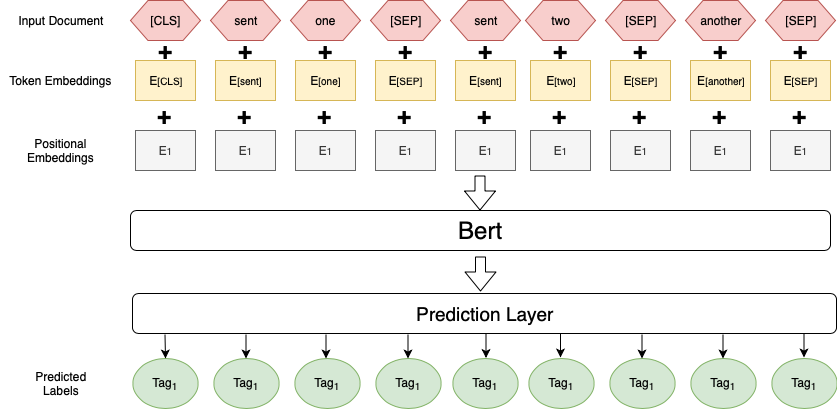
\includegraphics[width=\linewidth]{model}
	\caption{The overview of token-level tagging model. Note that comparing to \citet{bert-sum}, we only add [SEP] tokens instead of adding both [SEP] and [CLS], and we do not have interval segment embedding. }
	\label{fig:overview}
\end{figure*}

\section{Models}
We used Bert to extract contextual embedding and layered on top 2 different kind of prediction layers. An overview of the model architecture can be found at Figure \ref{fig:overview}

\subsection{Simple Linear Classifier} \label{simple-linear}
The first layer we tried is a simple linear layer on top of Bert following the original Bert paper \cite{bert}. This linear layer calculates the unnormalized score of how likely a source token is included in the target summary. Then, a sigmoid function is applied to each unormalized score to get the predicted score of token membership:
\begin{equation}
	y^{(i)} = \sigma(w^T x_j^{(i)} + b)
\end{equation} 
where $\sigma$ is the sigmoid function, $w$ is a learnable vector, $x_j^{(i)}$ is the bert encoding at the $j$th position in the $i$th source document.

\subsection{Transformer Layer}
Another architecture we tried is the transformer architecture introduced by \citet{attention}. We used the code accompanied by the paper\footnote{code can be found at \url{https://github.com/jadore801120/attention-is-all-you-need-pytorch}, we copied code from the transformer module and attention module.}. Formally, we calculate the multi-headed self attention as follows:
\begin{align}
	Q_j &= EW^{[q]}_j + b^{[q]}_j\\
	K_j &= EW^{[k]}_j + b^{[k]}_j\\
	V_j &= EW^{[v]}_j + b^{[v]}_j\\
	A_j &= \text{Softmax}(\frac{Q_jK_j^T}{\sqrt{d}}) V_j\\
	A &= A_j W^{[a]} + b^{[a]}\\
\end{align}
Essentially, we pass the Bert encoding $E$ into 3 linear layers and calculate the softmax of the dot product of two of the layers divided by the square root of the dimension of bert hidden size $d$. This calculates the self attended encoding for a single head $j$. Here, all $W$'s and $b$'s are learnable parameters and $E$ is the $n\times d$ last hidden layer output from Bert where $n$ is the number of tokens in the source document. $W^{[q]}_j$, $W^{[k]}_j$ are both $d\times h$ where $h$ is a tunable hyper parameter. $W^{[v]}_j$ is a $d\times d$ matrix. $W^{[A]}$ is a $d \times d\cdot\text{\{number of heads\}}$ matrix used to forward the attention from all heads into a fixed shape. In addition to self attention, we included residual connection by adding the Bert hidden layer $E$ with the attended output $A$ to produce the final output. Then, we added on top the same linear layer as described in section \ref{simple-linear} to find the predicted score of token membership.

Regardless of the prediction layer architecture, the model is then trained with binary cross entropy loss:
\begin{equation*}
	L^{(i)} = \sum_j y^{(i)}_j \log\hat{y}^{(i)}_j + (1-y^{(i)}_j)\log(1-\hat{y}^{(i)}_j)
\end{equation*}

where $y^{(i)}_j$ is the true label of whether the token at source position $j$ is included in the target summary or not, and $\hat{y}^{(i)}_j$ is the unnormalized score outputted by the model.

Note that since Bert already use the same kind of attention architecture, we hypothesize that by training a brand new attention layer we would perform better than only using the pretrained embeddings. Results about this would be discussed in a later section.

\begin{table*}[t!]
	\centering
	\begin{tabular}{c|ccc}
		Model                & Rouge-1 & Rouge-2 & Rouge-L \\ \hline
		Seq-Seq \cite{lead}*              & 35.46   & 13.30   & 32.65   \\
		Pointer-Generator \cite{pointer-generator}*    & 39.53   & 17.28   & 36.38   \\
		Bottom-up \cite{bottom-up}*            & 41.22   & 18.68   & 38.34   \\
		DCA \cite{dca}*                  & 41.69   & 19.47   & 37.92   \\
		HSSAS \cite{al2018hierarchical}*                & 42.3    & 17.8    & 37.6    \\
		Bertsum \cite{bert-sum}*              & 43.25   & \textbf{20.24}   & 39.63   \\ \hline
		LEAD-3 Baseline (ours) & 38.21 & 15.45 & 32.39 \\
		Oracle				& 88.11 & 76.37 & 85.52 \\
		Bert-tokenSum Simple    & 44.80   & 18.57   & 39.70   \\
		Bert-tokenSum Attention & \textbf{44.91}   & 18.21   & \textbf{39.81 }
	\end{tabular}
	\caption{F1 test ROUGE scores. Model names with a [*] next to them are results taken from their corresponding paper. Oracle scores included for reference (refer to section 4 for explanation) Again, the comparisons shown here require further verification since we may have used different tokenization strategy (notably, the target summaries are all lower cased).}
	\label{table:results}
\end{table*}

\subsection{Inference}
At inference time, we will chose a threshold and select all the tokens with a predicted score above that threshold. Then, we will concatenate all the tokens together, and do some post processing to remove any bert-specific tokenization constructs (such as [CLS] and [SEP]). Since we do not want target summaries to be too long (or simply include all the tokens in the document), the predicted summary is truncated to 120 tokens before removal of bert-specific tokens.



\section{Experiments}
To use Bert as our token level encoder, we must format our source documents into a form that Bert understands. We first tokenized the source document using Stanford Core NLP following \citet{pointer-generator} with preprocessing code (\href{https://github.com/abisee/cnn-dailymail}{link}) accompanied with the paper. Then, we added [SEP] tokens in between source sentences and [CLS] token in front of the whole document. Then, we used BertTokenizer from the HuggingFace implementation of Bert in Pytorch (\href{https://github.com/huggingface/pytorch-pretrained-BERT}{link}) to tokenize the source sentences and convert them to indices into the token embeddings. Then, we tokenized the gold summary with Bert and used it to generate the tags for each source token as described in section 4. Source document is truncated to 510 tokens and target summary is truncated to 110 tokens, slightly higher than \citet{bert-sum}. Note that we also tokenize the target summary according to Bert (adding [SEP] and [CLS] tokens), and removed these tokens during ROUGE score calculation. The reason is that we believe including [SEP] tokens would help inform the model the end of sentences. However as a side effect, our target summary might look different from other paper's "gold" summary, so results from this report should be handled with care when comparing it against other papers. We implemented our own training and evaluation framework, borrowing from a course project that we have done before. 

Training each model took about 25 hours on a single Nvidia V100 GPU and exhausted all of our available Google and AWS credits. We trained the model around 1,400,000 steps (around 5 epochs), and evaluating the model at 100,000 step at a time on the evaluation set. Then, we pick the model with the lowest dev loss for further evaluation and testing.

\subsection{LEAD-3 Baseline}
Since re-implementing other papers with our own tokenization and task definition is infeasible given the amount of time, we additionally include the popular LEAD-3 baseline, which is essentially using the first 3 sentences from the source document as the predicted summary. This method is widely used and compared against in almost all document summary papers, and serves as a simple yet very powerful baseline. \citet{bottom-up} also established this baseline and showed that their model only slightly improves upon this baseline while attaining state-of-the-art results.

Since many documents have "filler sentences" in the beginning of the document indicating the author, date, and location of the article, we start with finding the first sentence that has more than 10 tokens and include the next 2 sentences that immediately follows that. The generated target summaries have on average 386 characters comparing to 296 in the gold summaries.
%\begin{table*}[t!]
%	\centering
%	\begin{tabular}{|c|c|c|c|c|c|c|c|c|c|c|}
%		\hline
%		\multirow{2}{*}{Threshold} & \multirow{2}{*}{Length} & \multicolumn{3}{c|}{Rouge-1}                    & \multicolumn{3}{c|}{Rouge-2}                     & \multicolumn{3}{c|}{Rouge-L}                     \\ \cline{3-11} 
%		&                         & P             & R              & F1             & P              & R              & F1             & P              & R              & F1             \\ \hline
%		-2.5                       & 498                     & 37.27         & \textbf{55.02} & 43.50          & 15.14          & \textbf{25.48} & 18.45          & 34.43          & \textbf{50.90} & 37.02          \\ \hline
%		-1.7                       & 418                     & 41.48         & 51.44          & \textbf{44.84} & 16.34          & 22.99          & \textbf{18.55} & 38.75          & 48.06          & \textbf{39.72} \\ \hline
%		-0.5                       & 54                      & \textbf{57.9} & 13.5           & 19.93          & \textbf{26.25} & 6.01           & 8.6            & \textbf{56.02} & 12.96          & 13.65          \\ \hline
%	\end{tabular}
%	\caption{Different ROUGE scores for different thresholds of the model with only a simple linear classifier on top of Bert (evaluated on the dev set). Thresholds are on unormalized scores (before sigmoid function). Bolded results are the highest values of the metric across all thresholds. The middle threshold is chosen as the threshold with the highest F1 score. P denotes precision, R denotes recall, F1 denotes F1-score (duh)}
%	\label{table:threhold}
%\end{table*}

\begin{figure*}[t]
	\centering
	\begin{minipage}{.33\linewidth}
		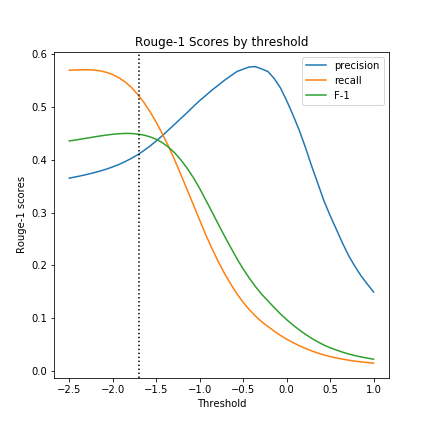
\includegraphics[width=\linewidth]{plots/rouge-1.png}
	\end{minipage}
	\begin{minipage}{.33\linewidth}
		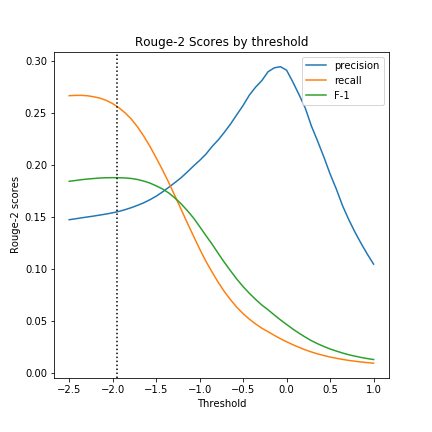
\includegraphics[width=\linewidth]{plots/rouge-2.png}
	\end{minipage}
	\begin{minipage}{.32\linewidth}
		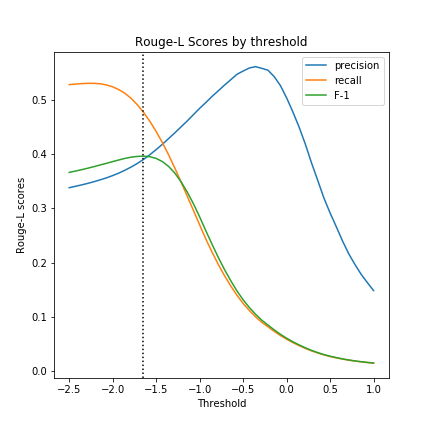
\includegraphics[width=\linewidth]{plots/rouge-L.png}
	\end{minipage}
\caption{The precision, recall, and F-1 score of various Rouge metrics with different thresholds. The dotted line shows the threshold with the highest F-1 score}
\label{fig:threshold}
\end{figure*}


\section{Results and Discussion}
This section reports the results from our experiments. Both models outperformed the popular LEAD-3 baseline, and we also arguably achieved state of the art results.\footnote{This statement requires further verification by re-implementing the other author's models using the same tokenization} Table \ref{table:results} shows the comparison between our model and models from several notable previous papers. The current state of the art result is from Bertsum, and we have shown that our model could potentially improve that result by nearly 1.75 Rouge-1 scores. Still, it does not do better in Rouge-2 scores, and achieved similar results in Rouge-L scores. The reason is that we are ultimately predicting sub-sequences instead of sub-strings of the source documents, so we do not perform as well in terms of whole sentence extraction comparing to sentence-selection style models. However, we do better in unigram overlap F-1 since sub-sequence selection allows us to select tokens across multiple sentences instead of having to select exactly 3 whole sentences.
 \begin{table*}[t!]
	\centering
	\begin{tabular}{@{}|l|l|@{}}
		\hline
		\textbf{Predicted (-0.6)} & 
		\begin{minipage}{5in}
			cambridge dr markus kuhn from university of cambridge said the sim could have been replaced long ago . he believes alternatives include typing in a user identifier and password directly into a phone . .
		\end{minipage}\\ \hline
		\textbf{Predicted (-1.8)} & 
		\begin{minipage}{5in}
			the . but sims devices . a cambridge computer science experts believes the small microchips ' days are and should be phones in the online accounts . dr markus kuhn from the university of cambridge said the sim could have been replaced long ago . he believes alternatives include typing in a user identifier and password directly into a phone . sim could with id and password into the phone is to access wifi of cambridge . or qr codes 3d are more alternative for smartphones with cameras app can . the to . . ' believes sims with passwords software it . they .
		\end{minipage}\\ \hline
		\textbf{Gold} &
		\begin{minipage}{5in}
			dr markus kuhn said the sim could have been replaced a long time ago . he believes one alternative could be typing in a user identifier and password directly into a phone - like we do with wi - fi networks . or details could be encoded in qr codes photographed by a phone camera . the university of cambridge lecturer also believes the time is right to switch because of recent advances in cryptographic techniques .
		\end{minipage}\\ \hline
	\end{tabular}
	\caption{An example of predicted and gold summaries when we use low and high thresholds.}
	\label{table:threshold-examples}
\end{table*}

\subsection{Model Differences}
To evaluate model differences, we trained the models independently, and selected the best threshold that maximizes the Rouge-1's F1 score (thus we are optimizing over Rouge-1 scores). Then, we use the corresponding threshold on the test set to obtain the results in table \ref{table:results}. Notice that with a brand new self-attention layer, our model does slightly better in Rouge-1 and Rouge-L scores, but slightly worse in Rouge-2 scores. However, we believe that this is all within the margin of error, and the two models are essentially equally high performing. We thus cannot definitively say that the Bert + self attention model is definitely better.

\subsection{Threshold}
Threshold selection is integral to the success of the model. Here, we discuss how thresholds influences each metric, and how varying thresholds actually allows us to construct different type of summaries.

Figure \ref{fig:threshold} shows the difference in scores when we vary the thresholds. With increasing thresholds we have a reduction in the size of the generated summary and thus a decrease in uni-gram, bi-gram, and longest common sequence recall, since less of those tokens will be included in the predicted summary. Notice that the recall flattens or even decreases when threshold is too low. This is because we truncated predicted summaries to 120 tokens, and thus when the threshold is too low we simply included all of the tokens in the source document truncated to 120 tokens. Another effect is that the precision goes up significantly until capping out at around -0.5 to 0. This shows that the model is better at confidently picking the relevant words that are indeed included in the target summary up until a certain threshold, then slowly stopped including vital words.

Another promising result is that we can use different thresholds to get different level of summaries. For example, as shown in table \ref{table:threshold-examples}, setting threshold to be -0.6 will yield a 2 sentence summary, which also appeared in the gold summary. Setting threshold to -1.8 gives a more verbose and complete version of the summary, albeit less grammatically correct and fluent than the gold summary. However, this particular example does not generalize to other document. Thus, setting the threshold high enough could be used as a content selector/keyword extractor instead of a summarizer.

\subsection{Model Weakness}
Although we achieve fairly high ROUGE scores, it only shows that our model is very good at picking words from the source document to include in the summary, but still it has great trouble ordering the words correctly or generate coherent summaries. Comparing to results from generative methods such as \citet{pointer-generator}, our summarizer is unable to achieve the level of coherency as them. Looking at the example from table \ref{table:threshold-examples}, the long summary generated have most of the key tokens in the gold summary, such as "wifi", "camera", et. but it is unable to order them or fill in other words to generate a coherent summary. Thus, token selection itself is not enough, and ordering and filling in other words is also necessary to generate a coherent summary.

Another thing we have noticed is that our summarizer is very good at selecting the correct words so long as the target summary mostly contain tokens in the beginning of the document. The longer the document the harder it is for our summarizer to pick the right tokens. This has been a well researched problem in long document tasks, both in QA systems and translation systems with currently no 100\% sure fire way to solve it. 

The choice of using Bert is also not optimal since Bert is pretrained on a masked token prediction task with 2 sentences. Thus, it limits the model's ability to generalize it to longer multi-sentence document like the one we have. We did not include the segment interval embedding for this reason, but we could borrow the interleaving interval idea from \citet{bert-sum} in a later work.

\section{Conclusion and Future Works}
This work casts the document summarization problem as a sub-sequence tagging problem and experimented using Bert with other neural networks to predict source token membership in target summary. We introduces a novel sub-sequence tagging method and showed that with a simple linear layer on top of Bert we are able to achieve better results than other papers, including beating state of the art extractive methods. However, we need to evaluate this statement further by re-implementing the models of previous papers with our tokenization strategy to confirm results. 

There are several things that we could try in the future. For example, we currently only have a basic content selector. In reality, we could re-implement the bottom-up summarizer \cite{bottom-up} with our own content selector and observe results. The bottom-up summarizer combines both extractive and abstractive method, and since our content selector performs better than theirs, we might be able to improve their result. Another thing we could try out is using Open GPT or a Transformer-XL architecture. These new architectures have shown to perform better on longer sequence tasks.

\section{Authorship}
The project is completed by Haojun Li only (me myself and I) without contribution from anyone else. I take full responsibility for my work.

\newpage
\bibliography{paper}
\bibliographystyle{acl_natbib}

\end{document}
